\section{Analisi esplorativa}

Il passo di data integration che abbiamo svolto è stato effettuato in modo da preparare un dataset che non necessitasse di ulteriori modifiche dal punto di vista degli attributi, in grado di poter creare fin da subito un modello da sottoporre agli algoritmi di Machine Learning. Sono stati eliminati solamente gli attributi relativi ai nomi degli attaccanti e dei difensori, utilizzati solamente per il matching durante l’integrazione a causa dell’assenza di un id univoco.

\par
Infatti, è stata fatta sin dal principio un’analisi degli attributi in questa direzione. Il dataset integrato risultante possiede per ciascuno dei 128 000 tiri informazioni relative al tiro stesso, prese dal dataset Shot logs, oltre ad informazioni supplementari relative sia agli attaccanti che ai difensori, prese dal dataset Season stats. Non sono stati inclusi alcuni attributi da entrambi i dataset.
\par

In Shot logs sono stati esclusi alcuni attributi (descritti in Tabella 2.1) riguardanti la partita come \texttt{W}, \texttt{Final margin} e \texttt{Matchup} perché ritenuti non incidenti per le sorti di un tiro a canestro. Inoltre, sono stati ritenuti esclusi alcuni attributi riguardanti il tiro a canestro come \texttt{Period} e \texttt{Game clock}, che abbiamo ritenuto ridondanti in quanto già presente l'attributo \texttt{Shot number}, così come non significativo è stato valutato l'attributo \texttt{Pts type} in quanto deducibile dall'attributo \texttt{Shot distance}. In Seasons stats, per lo stesso motivo, sono stati esclusi decine di indici statistici non determinanti, oltre agli attributi (descritti in Tabella 2.2) come \texttt{Games} e \texttt{MP}.

\par
Sono assenti, invece, alcune informazioni più specifiche inerenti alla partita, come ad esempio la precisa posizione dei giocatori sul rettangolo di gioco piuttosto che l’effettiva distanza tra essi, oppure la stabilità dell’attaccante durante il tiro (o durante la difesa nel caso del difensore). Queste e altre dinamiche di gioco potrebbero essere utili per creare modelli più approfonditi in modo da fornire predizioni meno superficiali.

\par
I valori da predire sono distribuiti in modo non uniforme. Il 55\% (70157 record) sono tiri \textit{missed}, mentre il 45\% (57900 record) sono tiri \textit{made}.

\begin{figure}
\caption{test}
\fontsize{9pt}{1em}
	\includegraphics[width=\linewidth]{shot_result}
\end{figure}

\par
Per effettuare un'analisi esplorativa del dataset abbiamo trainato il modello con un numero ridotto di record (25 000) in modo da poter valutare il contributo informativo di ciascun attributo con un numero sufficiente di dati a disposizione.

\begin{figure}
\caption{test}
\fontsize{9pt}{1em}
	\includegraphics[width=\linewidth]{importance}
\end{figure}

\par
Come è possibile vedere nella Figura, i tre attributi con maggior contributo informativo sono \texttt{shot\_dist}, \texttt{close\_def\_distance} e \texttt{dribbles}. Abbiamo quindi plottato su un piano cartesiano \texttt{shot\_dist} e \texttt{close\_def\_distance} ed il risultato è visibile nella figura successiva.

\begin{figure}
\caption{test}
\fontsize{9pt}{1em}
	\includegraphics[width=\linewidth]{plot_shot_dist_def}
\end{figure}

Il grafico è stato interpretato considerando due regioni: la regione con prevalenza \texttt{made}, ossia quella compresa tra $[0, 10]$ nell'asse delle ascisse e $[5, 40+] $ nell'asse delle ordinate, e la regione con rpevalenza \texttt{missed}, ossia quella compresa tra $[25, 40]$ nell'asse delle ascisse e $[0, 20] $ nell'asse delle ordinate.
Queste due regioni sono riscontrabili nel mondo reale: i tiri effettuati dal pitturato, seppur con il difensore alle calcagne, hanno una probabilità di essere messi a segno molto alta. I tiri effettuati dalla distanza, invece, sono di notevole difficoltà e la probabilità di fallimento è alta anche se l'attaccante è un giocatore estremamente efficiente ed affidabile.

\par
Un quarto attributo con contributo informativo elevato è \texttt{PER\_attack}. Questo e l'interpretazione precedente porta a valutare una correlazione tra la \texttt{shot\_dist} e il ruolo degli attaccanti.

\begin{figure}
\caption{test}
\fontsize{9pt}{1em}
	\includegraphics[width=\linewidth]{shot_dist_with_position}
\end{figure}

Il grafico mostra che C, ovvero il componente della squadra che domina il pitturato, tira in media da una distanza inferiore ai 10 piedi, seguito da PF. Un'interpretazione del grafico precedente (da numerare) e questo grafico mostra che i giocatori in questo ruolo prendono tiri meno rischiosi. Non abbiamo a disposizione informazioni relative a peso e altezza, ma una ricerca correlata mostra che in media i giocatori in questi due ruoli sono anche quelli più prestanti dal punto di vista fisico, che soffrono meno il contatto con l'avversario e riescono a raggiungere più facilmente il canestro utilizzando prettamente queste loro caratteristiche.
Al contrario, gli altri tre ruoli (PG, SF e SF) tirano da una distanza che si aggira intorno ai 15 piedi. Sono meno prestanti dal punto di vista fisico ma solitamente con un'abilità al tiro maggiore, che li porta a prendere anche tiri rischiosi e più difficili, portando ad abbassare le loro statistiche.

\begin{figure}
\caption{test}
\fontsize{9pt}{1em}
	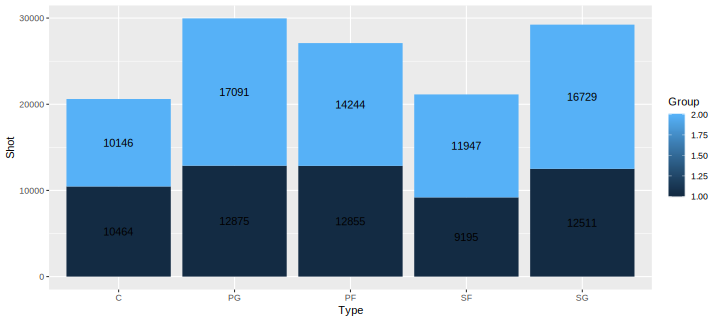
\includegraphics[width=\linewidth]{made_missed_barplot}
\end{figure}

Questo grafico conferma il discorso fatto precedentemente. PF ha una percentuale di missed pari a 0.53; ancora più bassa la percentuale di missed per C, pari a 0.49: l'unico ruolo ad avere un numero di tiri made maggiori rispetto ai missed ma anche la posizione con il numero minore di tiri effettuati.
Tutti e tre i ruoli più delicati (PG, SF, SG) hanno una percentuale di missed pari a 0.57, confermando la regola.






